\documentclass[11pt]{beamer}
\usepackage[utf8]{inputenc}
\usepackage[T1]{fontenc}
\usepackage{lmodern}
\usepackage[english]{babel}
\usepackage{amsmath}
\usepackage{amsfonts}
\usepackage{amssymb}
\usepackage{graphicx}
\usetheme{Madrid}
\begin{document}
	\author{Nayan Jani\\
		Christopher Odoom\\
		Denis Folitse\\
		Animesh Sengupta}
	\title{\bf{A Quasi-Poisson Regression Analysis:\\}
     \subtitle{Goals in Football, What contributes to them? }}
	%\subtitle{}

	\institute{\textbf{   University of Massachusetts, Amherst }}
	%\date{}
	%\subject{}
	%\setbeamercovered{transparent}
	%\setbeamertemplate{navigation symbols}{}
	\begin{frame}[plain]
		\maketitle
	\end{frame}
 
  \begin{frame}
 
		\frametitle{Outline}
\tableofcontents
\section{Background of study}
\section{Motivation}
\section{Objectives}
\section{Methodology}
\section{Descriptive Analysis}
\section{Comparative study}
\section{References}
  
  \end{frame}
  
  \begin{frame}
  \color{blue}
    \begin{center}
        \Huge\textbf{Background of study}
    \end{center}
	\end{frame}
\begin{frame}{Background of study}	
		\frametitle{Background of study}

  \begin{itemize}
  \setlength\itemsep{3em}
  \item Football has become a part of the world and is one of the biggest source of entertainment in the world. It has created job and opportunities to people all over the world..
  \item There are five major football leagues in the world; English premier league, German BundesLiga, Spanish Laliga, Italian Serie A and France League one.
  \item Football supporters in the various leagues all over the world always claim that, their league is the difficult one among all the five major leagues, is this claim true?.
  
  \end{itemize}
		
\end{frame}

\begin{frame}
\color{blue}
    \begin{center}
        \Huge\textbf{Motivation}
    \end{center}
	\end{frame}
	
	\begin{frame}{Motivation}
 
		\frametitle{Motivation}
   \textbf{Arguments:}
  \begin{itemize}
  \setlength\itemsep{1.5em}
 
      \item If teams score lot of goals week in week out in a league, that leagues quality is brought to question. Goes as far as labeling the league a "Farmers League"
      \item Goal scoring stats has been used a lot of late to determine how good an attacking player performs. 
      \item Unfortunately, Due to this labeling of some leagues as having a low quality, Some players are still undermined no matter the number of goals they bang week in week out.
      \item Other times, defenders are blamed to be too poor.
      
 \end{itemize}
	\end{frame}

 \begin{frame}
 \color{blue}
    \begin{center}
        \Huge\textbf{Objectives}
    \end{center}
	\end{frame}

	\begin{frame}{Objectives}
		\frametitle{Objectives}
      \textbf{Main Objective:}\\
      \setbeamertemplate{itemize items}[ball]
      \begin{itemize}
          \item  Does the type of league determine the number of goals scored per season combined with other variables?\\
      \end{itemize}
         
        \textbf{Specific Objectives:}
		\begin{enumerate}
		 
			
			\item Determine if there is a significant difference in goals across the 5 major leagues.
			
			\item Determine if there are other predictors that are associated with the goals other than the different leagues.
			
		\end{enumerate}
	\end{frame}


\begin{frame}
\color{blue}
    \begin{center}
        \Huge\textbf{Methodology}
    \end{center}
	\end{frame}
	\begin{frame}{Methodology}
		\frametitle{Data}
  \begin{itemize}
  \setlength\itemsep{3em}
		\item We used data from the
		2021-2022 season for five major leagues: EPL, La Liga, Bundesliga, Ligue 1 and Serie A in the analysis.
        \item The data comprise of 98 observations and 17 variables.
        
        \item The data was pulled from \url{ https://fbref.com} 
		 

	\end{itemize}

 \end{frame}
 

 \begin{frame}{Variable Description}
 \includegraphics[scale=0.5]{"Screenshot (46).png"}
     
 \end{frame}
 
 \begin{frame}
\frametitle{Data Process}
	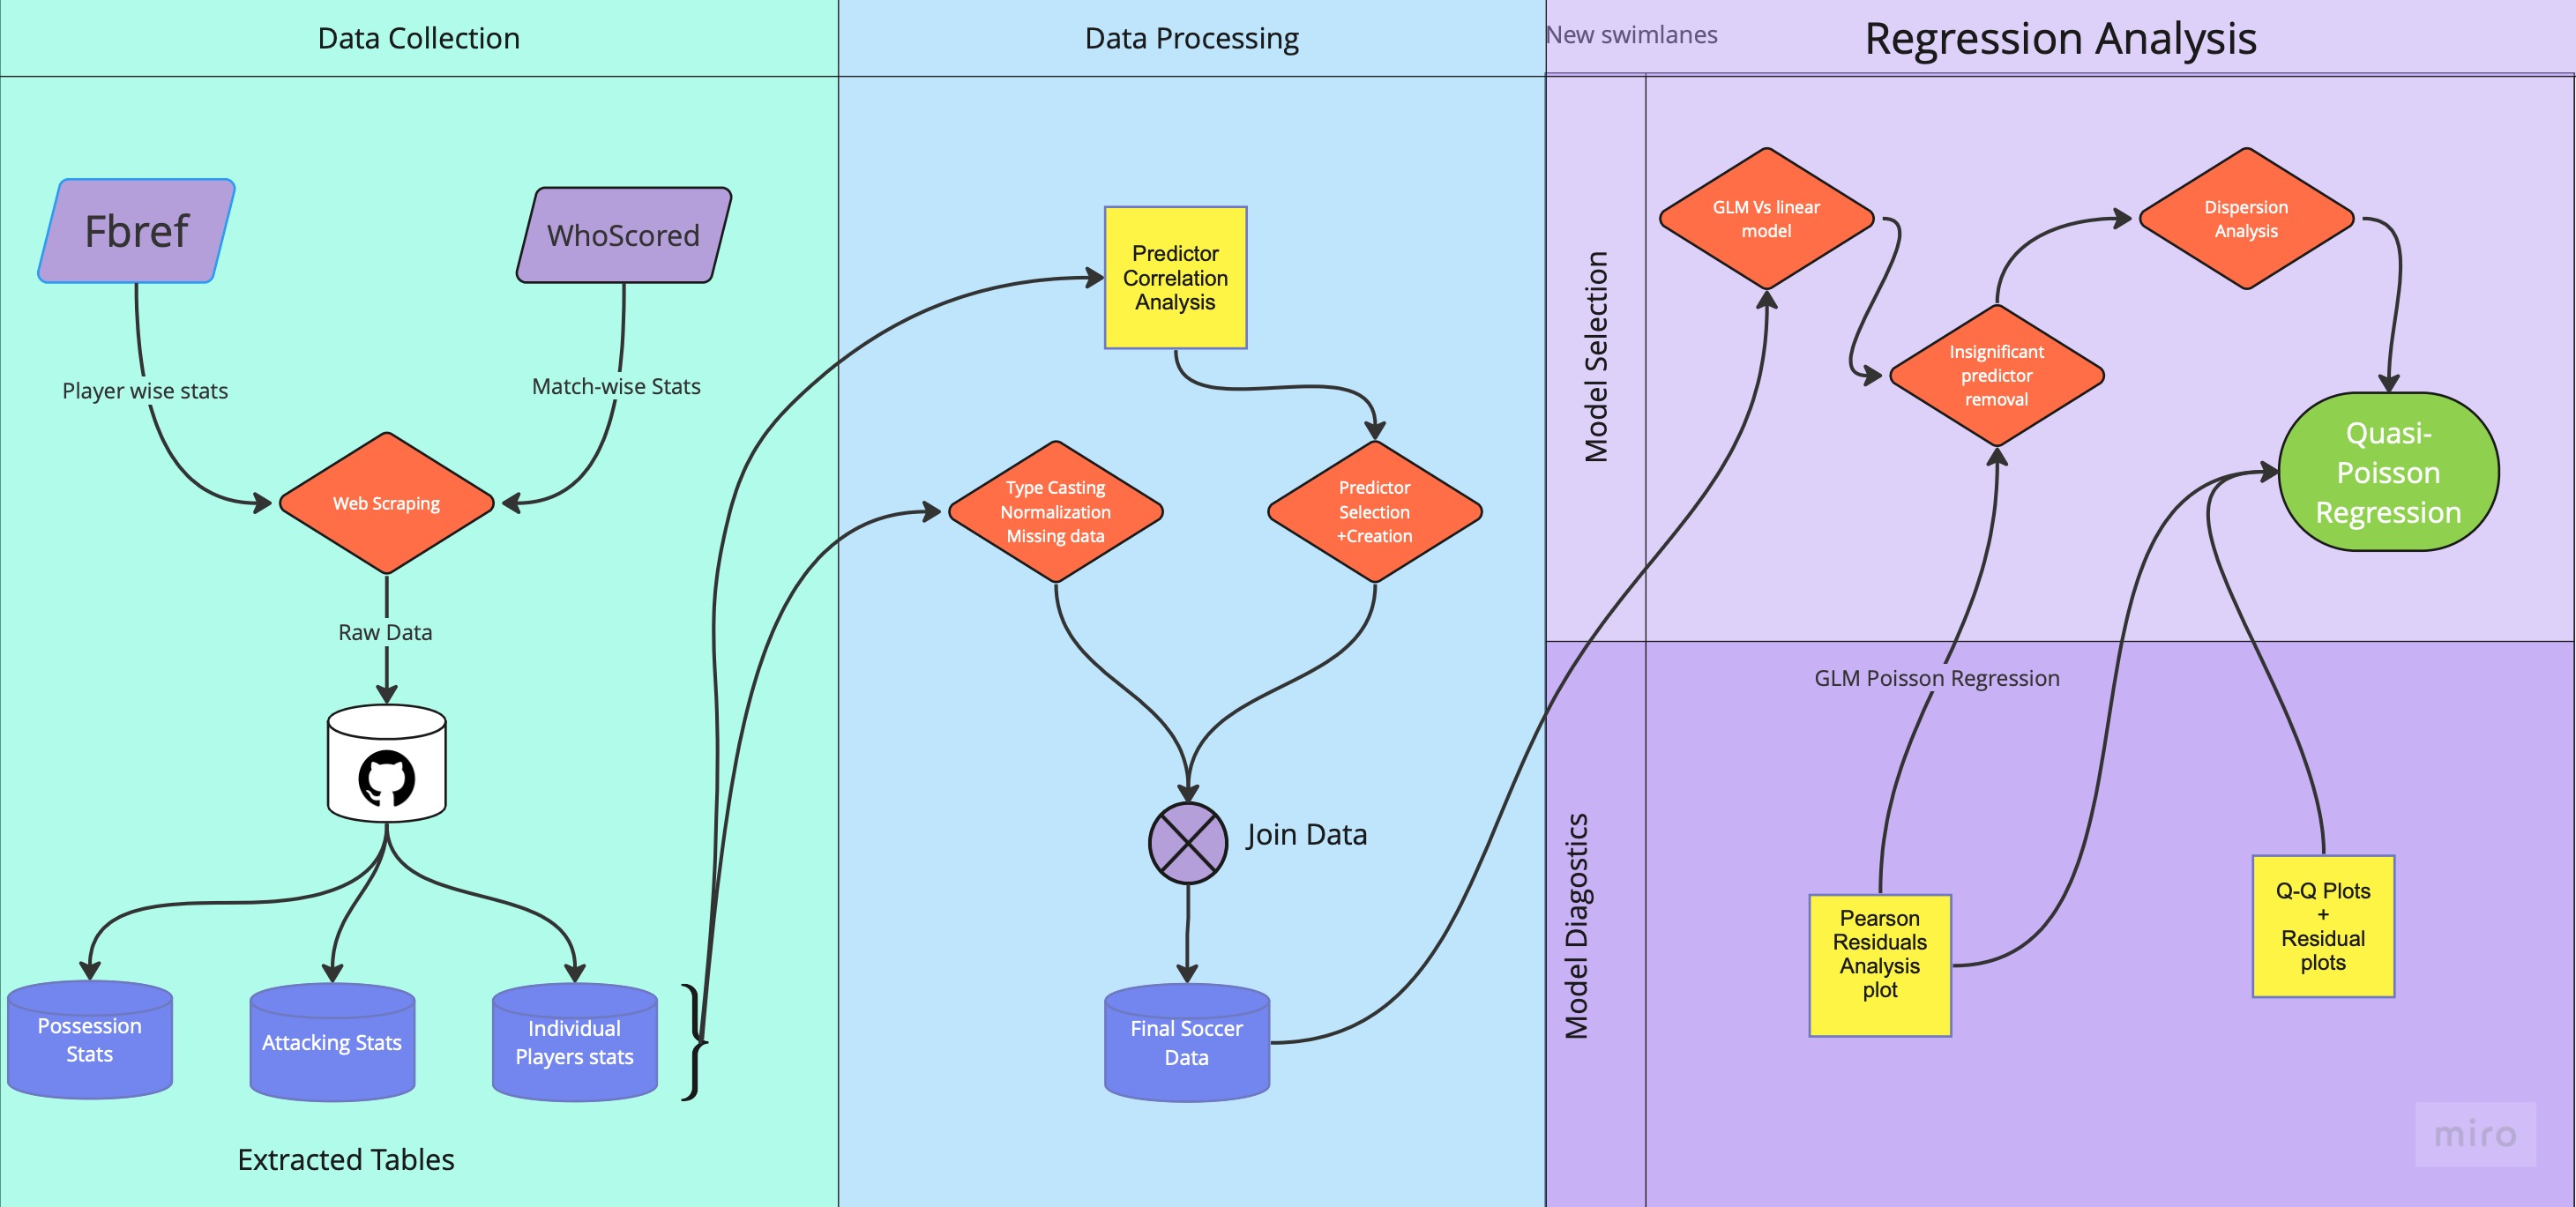
\includegraphics[scale=0.12]{STAT625-3.jpg}\\
		\figurename 1: Data Analysis flow chart

\end{frame}
\begin{frame}

	\frametitle{Poisson Regression}

    In Deciding for the model;
    
   

    \begin{itemize}
     \setlength\itemsep{2em}
    \item \textbf{Random Component:} The random component identifies the response variable and selects a probability for it. For our objectives, the response variable, No. of Goals is a COUNT variable that follows a Poisson distribution. 
    \item \textbf{Systematic component:} In here, this component help specifies the explanatory variables as a linear predictor. For each explanatory predictor, $i$, the linear predictors are given as; \[\beta_0+\beta^{'}_{i}X_{i}\]

    \item \textbf{Link Function:} We specify the function, $g(.)$ that connects the random and systematic component. i.e relating our expected response variable to the linear predictors. For our response: Since the expected No. of goals cannot be negative; we use the log link. 

 \end{itemize}
\end{frame}

\begin{frame}
     This give us the mathematical equation below:
	\[\log(E(no.Goals|X))= \beta_0+\beta^{'}_{i}X_{i}\]
	Alternatively, we can write it in an exponential form as:
	\[E(No.Goals|X)= e^{(\beta_0+\beta^{'}_{i}X_{i})}\]
	The method used here to estimate the paramters is the Maximum Liklihood estimator.	
	
\end{frame}

\begin{frame}
	\frametitle{Assumptions of Poisson Regression:}
	\begin{itemize}
        \item The response, no. of goals must be a count data.
		\item The number of goals must be scored in a fixed time.
		\item \[E(no.Gls|X) =Var(no.Gls|X)\]
	\end{itemize}
\end{frame}
\begin{frame}
	\frametitle{Estimation of parameter}
	The estimation method used here is the maximum likelihood estimation method.
	The procedure is briefly described below:
	Given the model:
	\[\lambda(x)= E(Y|X)= e^{\beta^{'}X}\]
	Here Y, the response follow a Poisson distribution, therefore we have
	\[P(y|x,\beta^{'})= \frac{\lambda(x)^y e^{-\lambda(x)}}{y!}\]   \[= \frac{e^{y \beta^{'}X} e^{-e^{\beta^{'}X}}}{y!}\]
	
	Now suppose we have  data set $(X,y)$ with n rows, then given an set of parameters $\beta$ the likelihood is given by
	\[L(\beta|X,Y)= \prod_{i=1}^{n} \frac{e^{y_i \beta^{'}X_i} e^{-e^{\beta^{'}X_i}}}{y_i!}\]
	The goal is to find $\beta$ which maximize this likelihood.
\end{frame}
\begin{frame}
    \frametitle{Model Diagnostic}
    To make sure the assumption \[E(no.Gls|X) =Var(no.Gls|X)\] is met, we used the dispersion parameter.
    This is given by:
    \[\hat{\phi}=\frac{1}{n-K}\sum_{i=1}^{n}\frac{(y_i-\hat{y_i})^2}{\hat{y_i}}\]
	where K is the number of parameters.\\
	such that
	\[Var(Y|X)=\hat{\phi}E(Y|X) \]
 This implies that if: 
 \begin{itemize}
	 \item $\hat{\phi}=1$ then the assumption is met and then we have Possion regression\\
	 \item $\hat{\phi}>1$ we have over-dispersion\\
	 \item $\hat{\phi}<1$ we have under-dispersion
  \end{itemize}

\end{frame}
\begin{frame}
	\frametitle{Pearson Residuals}
 \begin{itemize}
 \setlength\itemsep{3em}
	\item We also did a Pearson residual to diagnose/verify if the poission regression is appropriate.
  \item This weights the residuals and when plotted with the fitted points helps us determine if there is an issue with dispersion or not. This measure is computed with the formula below.
 \end{itemize}
	\[Pearson Residual=\frac{y_i-\hat{y_i}}{\sqrt{\hat{y_i}}}\]  
\end{frame}
\begin{frame}
	\frametitle{Quasi-Poisson}
 As the assumption is violated, what next?
 \begin{itemize}
	\item In this study we used a variant of Poisson regression called Quasi-Poisson Regression for our final model as a result of the violation of the assumption: \[E(no.Gls|X) =Var(no.Gls|X)\]
    \item The data is under-dispersed( the conditional variance is smaller than expected).
	\item This model factors in the  dispersion parameter which help solve the problem of under-dispersion.\textbf{ The reason for this model is to produce credible inference.} 
 \end{itemize}
	
\end{frame}
\begin{frame}
	\frametitle{Pearson Residuals}
 \begin{itemize}
 \setlength\itemsep{3em}
	\item The Pearson residual corrects for the unequal variance in the raw residuals by dividing by the standard deviation. The formula for the Pearson residuals is
 \end{itemize}
	\[Pearson Residual=\frac{y_i-\hat{y_i}}{\sqrt{\hat{\phi}\hat{y_i}}}\]  
\end{frame}

\begin{frame}
\color{blue}
    \begin{center}
        \Huge\textbf{Results}
    \end{center}
	\end{frame}
\begin{frame}{Descriptive Analysis}


	\frametitle{Histogram}
	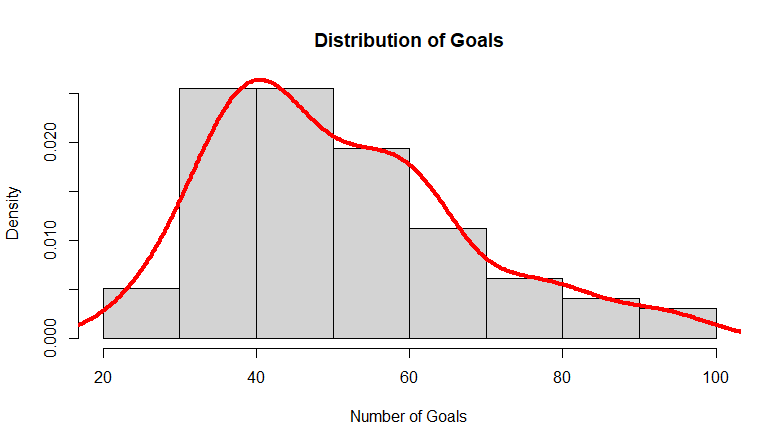
\includegraphics[scale=0.5]{gls1}\\
		\figurename 1: The plot show the goals distribution across the 5 Leagues
	\end{frame}
 \begin{frame}
	\frametitle{Boxplot}
	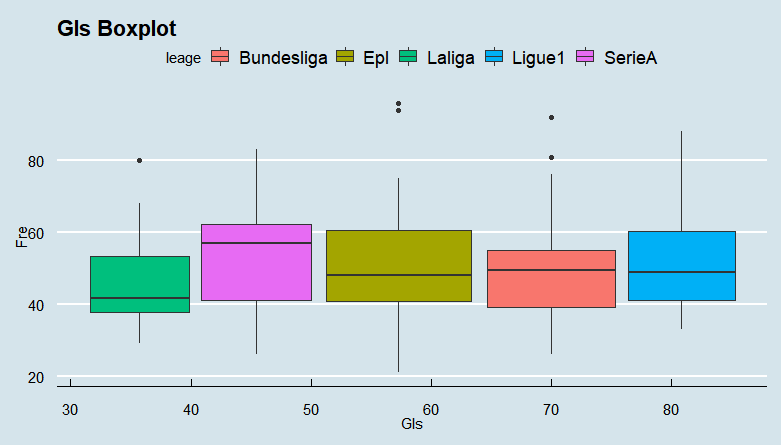
\includegraphics[scale=0.5]{Gls}\\
	\figurename 1: The plot show the goals distribution across the 5 Leagues
\end{frame}







\begin{frame}
	\frametitle{Linear Regression}
	% Date and time: Wed, Nov 30, 2022 - 7:08:42 PM
	\begin{table}[!htbp] \centering 
		\caption{Naive OLS Model (Multiple $R^2=0.9045$)} 
		\label{} 
		\begin{tabular}{@{\extracolsep{3pt}} ccccc} 
			\\[-3.8ex]\hline 
			\hline \\[-1.8ex] 
			& Estimate & Std. Error & t value & Pr(\textgreater \textbar t\textbar ) \\ 
			\hline \\[-1.8ex] 
			(Intercept) & $$-$14.943$ & $6.097$ & $$-$2.451$ & $0.016$ \\ 
			leageBundesliga & $5.375$ & $2.059$ & $2.610$ & $0.011$ \\ 
			leageLaliga & $$-$0.487$ & $1.872$ & $$-$0.260$ & $0.795$ \\ 
			leageLigue1 & $1.169$ & $1.895$ & $0.617$ & $0.539$ \\ 
			leageSerieA & $$-$0.614$ & $1.995$ & $$-$0.308$ & $0.759$ \\ 
			No.Pl & $0.133$ & $0.166$ & $0.802$ & $0.425$ \\ 
			SoT & $0.296$ & $0.034$ & $8.672$ & $0$ \\ 
			PK & $0.755$ & $0.273$ & $2.771$ & $0.007$ \\ 
			FK & $$-$0.147$ & $0.100$ & $$-$1.471$ & $0.145$ \\ 
			Att.3rd.T & $0.001$ & $0.001$ & $0.710$ & $0.479$ \\ 
			Succ.Drib & $$-$0.022$ & $0.012$ & $$-$1.785$ & $0.078$ \\ 
			ShortAT\_Pass & $0.001$ & $0.001$ & $2.102$ & $0.039$ \\ 
			NumAtt & $3.271$ & $0.626$ & $5.229$ & $0.00000$ \\ 
			\hline \\[-1.8ex] 
		\end{tabular} 
	\end{table} 

\end{frame} 
	

\begin{frame}{Descriptive Analysis}
	\frametitle{Results}
	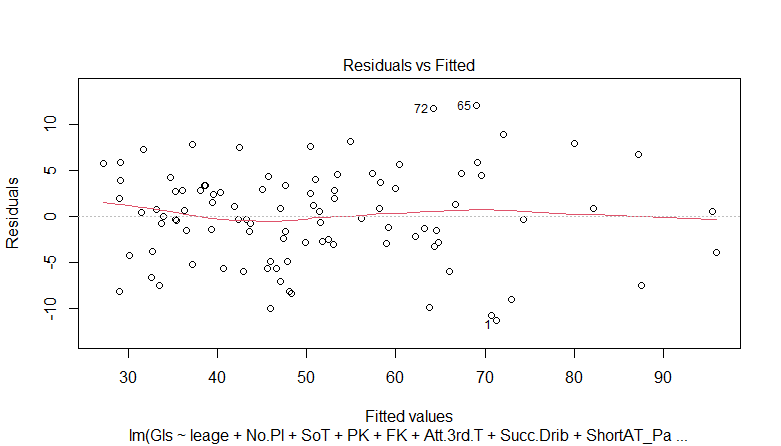
\includegraphics[scale=0.5]{gls2}\\
	\figurename 3: The residual plots for OLS
\end{frame}

\begin{frame}{Descriptive}
	\frametitle{Results}
	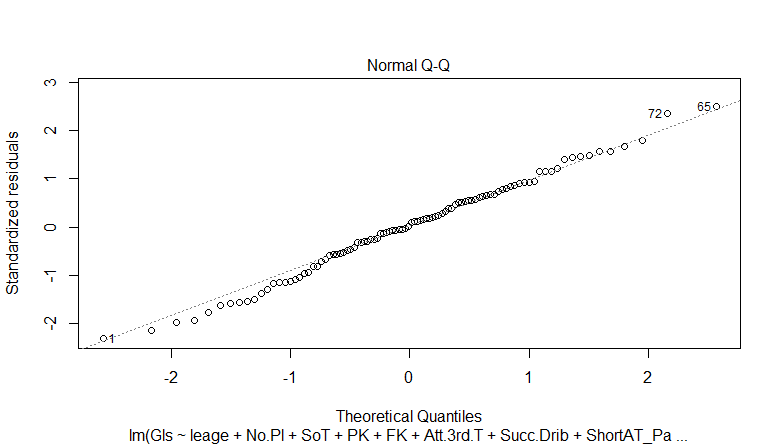
\includegraphics[scale=0.5]{gls3}\\
	\figurename 4: The QQ plot for OLS
\end{frame}
	


\begin{frame}
	\frametitle{Poisson Regression Output}
	\begin{table}[!htbp] \centering 
		\caption{Poisson Regression Output} 
		\label{} 
		\begin{tabular}{@{\extracolsep{5pt}} ccccc} 
			\\[-4.8ex]\hline 
			\hline \\[-1.8ex] 
			& Estimate & Std. Error & z value & Pr(\textgreater \textbar z\textbar ) \\ 
			\hline \\[-1.8ex] 
			(Intercept) & $2.853$ & $0.103$ & $27.592$ & $0$ \\ 
			leageBundesliga & $0.093$ & $0.053$ & $1.770$ & $0.077$ \\ 
			leageLaliga & $$-$0.007$ & $0.048$ & $$-$0.138$ & $0.890$ \\ 
			leageLigue1 & $0.036$ & $0.048$ & $0.742$ & $0.458$ \\ 
			leageSerieA & $0.004$ & $0.048$ & $0.089$ & $0.929$ \\ 
			SoT & $0.005$ & $0.001$ & $6.503$ & $0$ \\ 
			PK & $0.016$ & $0.007$ & $2.244$ & $0.025$ \\ 
			FK & $$-$0.003$ & $0.003$ & $$-$0.993$ & $0.321$ \\ 
			Att.3rd.T & $$-$0.00001$ & $0.00003$ & $$-$0.283$ & $0.777$ \\ 
			Succ.Drib & $$-$0.0005$ & $0.0003$ & $$-$1.655$ & $0.098$ \\ 
			ShortAT\_Pass & $0.00003$ & $0.00002$ & $1.885$ & $0.059$ \\ 
			NumAtt & $0.073$ & $0.015$ & $4.719$ & $0.00000$ \\ 
			\hline \\[-1.8ex] 
		\end{tabular} 
	\end{table}
Dispersion parameter $=1$ & Residual Deviance $= & Residual Deviance $= 58.267$$
\end{frame}


\begin{frame}{Diagnosis on Poisson regression}
	\frametitle{Residual Plot}
	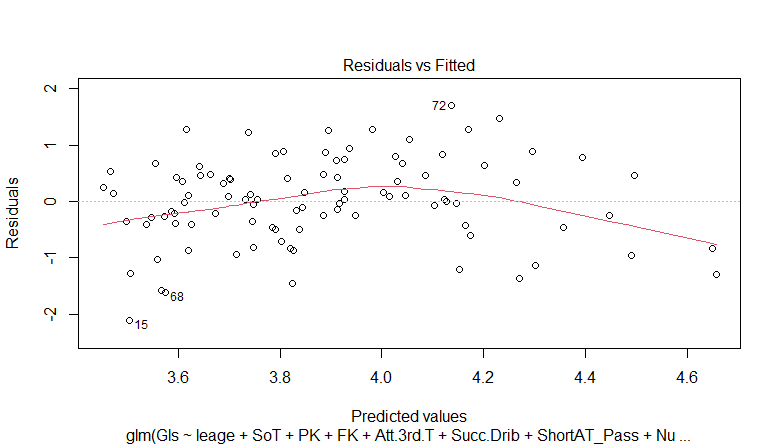
\includegraphics[scale=0.5]{gls4}\\
	\figurename 5: Residual Plot for Poisson Regression
\end{frame}
\begin{frame}{Diagnosis on Poisson regression}
	\frametitle{Pearson Residual Plot}
	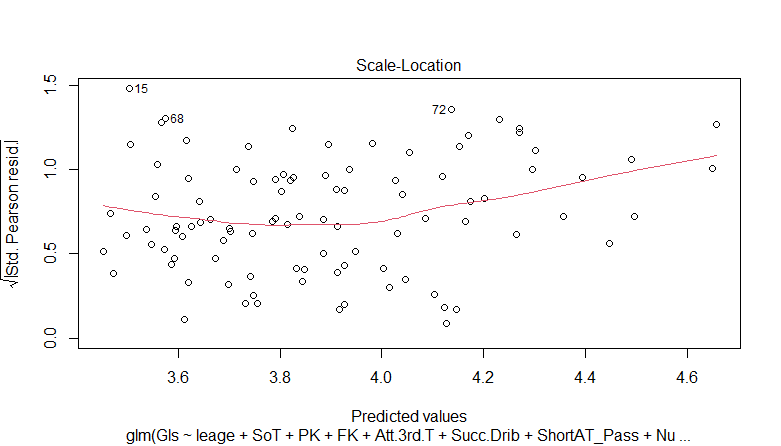
\includegraphics[scale=0.5]{gls5}\\
	\figurename 5: Pearson Residual Plots for Poisson regression
\end{frame}

\begin{frame}
	\frametitle{Quasi-Poisson regression Output}
% Date and time: Wed, Nov 30, 2022 - 7:04:09 PM
\begin{table}[!htbp] \centering 
	\caption{Quasi-Poisson regression } 
	\label{} 
	\begin{tabular}{@{\extracolsep{3pt}} ccccc} 
		\\[-4.8ex]\hline 
		\hline \\[-1.8ex] 
		& Estimate & Std. Error & t value & Pr(\textgreater \textbar t\textbar ) \\ 
		\hline \\[-1.8ex] 
		(Intercept) & $2.853$ & $0.084$ & $33.861$ & $0$ \\ 
		leageBundesliga & $0.093$ & $0.043$ & $2.172$ & $0.033$ \\ 
		leageLaliga & $$-$0.007$ & $0.039$ & $$-$0.169$ & $0.866$ \\ 
		leageLigue1 & $0.036$ & $0.039$ & $0.911$ & $0.365$ \\ 
		leageSerieA & $0.004$ & $0.039$ & $0.109$ & $0.913$ \\ 
		SoT & $0.005$ & $0.001$ & $7.981$ & $0$ \\ 
		PK & $0.016$ & $0.006$ & $2.754$ & $0.007$ \\ 
		FK & $$-$0.003$ & $0.002$ & $$-$1.219$ & $0.226$ \\ 
		Att.3rd.T & $$-$0.00001$ & $0.00002$ & $$-$0.348$ & $0.729$ \\ 
		Succ.Drib & $$-$0.0005$ & $0.0002$ & $$-$2.031$ & $0.045$ \\ 
		ShortAT\_Pass & $0.00003$ & $0.00001$ & $2.314$ & $0.023$ \\ 
		NumAtt & $0.073$ & $0.013$ & $5.791$ & $0.00000$ \\ 
		\hline \\[-1.8ex] 
	\end{tabular} 
\end{table}
Dispersion parameter$=0.6640285$. & Residual Deviance $= 58.267$
\end{frame}

\begin{frame}

% Date and time: Thu, Dec 01, 2022 - 3:29:58 AM
\begin{table}[!htbp] \centering
\caption{Exponent of the estimate sof Q-P output}
\label{}
\begin{tabular}{@{\extracolsep{5pt}} ccccc}
\\[-1.8ex]\hline
\hline \\[-1.8ex]
& Exponent Estimate  \\
\hline \\[-1.8ex]
(Intercept) & $17.343$  \\
leageBundesliga & $1.097$  \\
leageLaliga & $0.993$  \\

leageLigue1 & $1.036$  \\
leageSerieA & $1.004$ \\
SoT & $1.005$  \\
PK & $1.016$ \\
FK & $0.997$  \\
Att.3rd.T & $1.000$\\
Succ.Drib & $1.000$  \\
ShortAT\_Pass & $1.000$  \\
NumAtt & $1.075$  \\
\hline \\[-1.8ex]
\end{tabular}
\end{table}

\end{frame}

\begin{frame}{Diagnosis on Poisson regression}
	\frametitle{Effect Plot}
	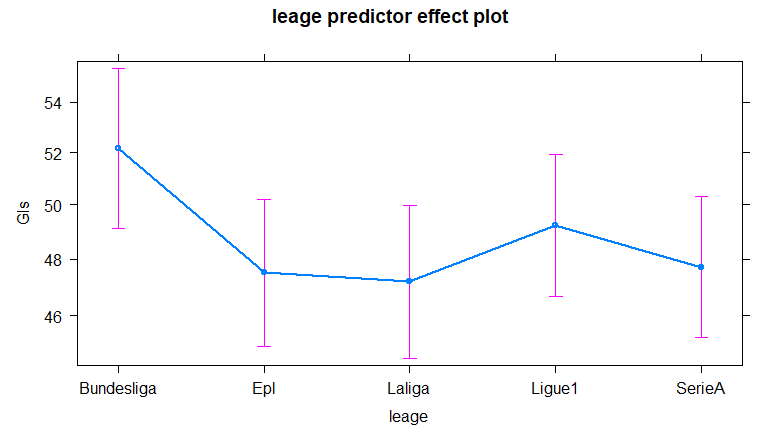
\includegraphics[scale=0.5]{gls6}\\
	\figurename 6: League Effect Plot for Poisson regression
\end{frame}


\begin{frame}{Diagnosis on Q-P regression}
	\frametitle{Pearson residual plot}
	\includegraphics[scale=0.5]{greatRplot.png}\\
	\figurename 7: Pearson Residual Plots for Q-P regression
\end{frame}
\begin{frame}
\color{blue}
    \begin{center}
        \Huge\textbf{Conclusion and Further Studies}
    \end{center}
	\end{frame}
\begin{frame}
	\frametitle{Conclusion and Further Studies}
 
 \begin{itemize}
   \setlength\itemsep{3em}
\item Based on our results we found that there was a significant difference in goals between Bundesliga and other leagues. Among the other leagues there is no significance in goals between them. 

\item Interestingly, we found that Shots on Target, Penalty Kicks, Successful Dribbles, Short Attacking Passes and Number of Attackers were significant. 

\item Further studies on this topic would include analysis of multiple seasons rather than just one season. We believe this would give us better results because it would lessen some of the outliers and biases that are present in just one season.
 
\end{itemize}	
\end{frame}

\begin{frame}{Reference}
\setlength\itemsep{3em}
	\frametitle{Reference}
 \begin{itemize}
 
\item Wallace, Jarryd & Norton, Kevin. (2013). Evolution of World Cup soccer final games 1966-2010: Game structure, speed and play patterns. Journal of science and medicine in sport / Sports Medicine Australia. 17. 10.1016/j.jsams.2013.03.016. 
\item \url{ https://fbref.com} 
	\end{itemize}
\end{frame}
\begin{frame}
\color{blue}
    \begin{center}
        \Huge\textbf{Thank You}
    \end{center} 
\end{frame}
\end{document}
